\chapter{Bayesian inference: From point estimates to probability distributions }\label{chapter:bayesian_inference}

This section presents an overview of the concepts in Bayesian inference used for the model estimation in the following chapters. It starts with a brief comparison between the Frequentist and Bayesian approaches. Then, it presents the theoretical foundations of Bayesian statistics and how these principles are transformed into a practical framework for parameter inference and modelling in the real world. 

This chapter is based on the ideas discussed by \citep{Lambert2018}, \citep{McElreath2016}, and \citep{Gelman2013} but is not intended to be an extensive review of the concepts. For further details, these sources are a good starting point. 

\section{The Bayesian paradigm: Frequentist vs Bayesian} 

Statistical inference has two “Schools of thought”: the Frequentist (or Classical) and the Bayesian approach. For frequentists, the data are assumed to be the result of an infinite number of repeated experiments with the same characteristics.  Then, the data are randomly sampled from a fixed and defined population, and any source of variation comes from that sampling process. Under this perspective, model parameters are assumed to be fixed but unknown values related to the population of interest, and the objective of inference is to calculate the best point estimate of the true value of the parameters given a data sample. 

In contrast, Bayesian statistics assume that data are observed and fixed quantities, and the source of variation comes from the uncertainty over the parameters. From this perspective, parameters are probabilistic values, and the objective of inference is to estimate the probability distribution of the model's parameters. Then, we use the data as evidence to update any prior belief about the underlying process. 

The debate about which approach is the best is exciting but long and almost philosophical; therefore, it is outside the scope of this document. However, as \citep{McElreath2016} points out, the Frequentist approach could make sense if the process of interest can be replicated multiple times, as in the case of many natural sciences (i.e., multiple controlled experiments in a laboratory). In contexts where the data collection can only be performed once, such as in many social sciences (i.e., democratic elections, population census), a Bayesian approach could be more aligned with the data nature. 

A quick overview of the Bayesian thinking framework is presented in \Cref{eq:bayesian_paradigm} \citep{Lambert2018}. The procedure begins with establishing prior beliefs about the process under analysis. Then, evidence (data) is gathered to update the prior beliefs using the model. The update is known as the posterior belief that includes the knowledge from both the priors and the data. 

\begin{equation}\label{eq:bayesian_paradigm}
    \text{prior} + \text{data} \xrightarrow{\ \ \ \ model\ \ \ \ } \text{posterior}
\end{equation}

\section{The basics of Bayesian inference} 

As the aim of statistical inference is to estimate the parameters of a model that recreates the process of interest, one of the objectives is to calculate the probability of getting the true parameters given the observed data or $P(\theta|data)$. However, as the true parameters are unknown, only the likelihood of the data being generated by the model parameters $P(data|\theta)$ can be calculated. 

According to\citet{Lambert2018}, both Frequentist and Bayesian inference aim to go from $P(data|\theta)$ to $P(\theta|data)$. While in the frequentist perspective, this transformation is not correctly carried out\footnote{The estimation is done by selecting the parameters that maximize the likelihood of obtaining our observed data.}, the Bayesian perspective applies the Bayes rule --\Cref{eq:bayes_rule}-- to properly transform the likelihood into a probability $P(data|\theta)\rightarrow P(\theta|data)$. The details of this transformation are reviewed in the following sections.

\vspace{3em}
\renewcommand{\eqnhighlightheight}{\vphantom{\hat{H}}\mathstrut}
\begin{equation}\label{eq:bayes_rule}
    \eqnmarkbox[lightBlue]{posterior}{P(\theta|data)} = \frac{\eqnmarkbox[lightGreen]{likelihood}{P(data|\theta)}\cdot\eqnmarkbox[lightRed]{prior}{P(\theta)}}{\eqnmarkbox[lightPurple]{evidence}{P(data)}}
\end{equation}
\annotate[yshift=2em]{above,left}{posterior}{posterior}
\annotate[yshift=2em]{above}{likelihood}{likelihood}
\annotate[yshift=1em]{above}{prior}{prior}
\annotate[yshift=-1em]{below}{evidence}{evidence}
\vspace{2em}

\subsection{Likelihood} 

One of the most important tasks when performing statistical inference is the choice of the model and its parameters. As the parameters are unknown to the modeller, the inference task is to estimate their value. One approach is to test different parameters on the chosen model and calculate the probability of getting the observed data for each set of values. The function that describes these probabilities corresponds to the \textit{likelihood function}. However, as this function is not a probability distribution, Bayesian statistics use Bayes theorem to convert this likelihood into a proper probability distribution. 

When defining the model, intrinsically, the data generation process is considered. Therefore, the likelihood includes the evidence and all the assumptions about the process. The higher the likelihood\footnote{In practice, the likelihood is transformed into the log-likelihood to ease the computation. This transformation also modifies the optimization process into a minimization. However, both approaches yield the same results.}, the better the estimation of our true parameter distributions. Given the directionality of the Bayesian thinking process $prior+data\rightarrow posterior$, the model definition is one of the most important factors in Bayesian inference. If the model choice does not represent the data generation process, no matter the prior selection, the inference process will fail to produce parameters that represent the reality. 

\subsection{Prior }

Also known as prior belief, it is the distribution or group of distributions\footnote{There is one prior for each model parameter.} representing previous knowledge of the process under study. This distribution encodes the existing knowledge and the modeller's uncertainty of the model parameters. 

In some cases, the problem is widely studied, and there is enough evidence about the possible values of the model parameters. In other cases, there is no previous evidence about the process. In the former case, the modeller is more confident about the expected value of the model parameter and can approximate the shape and location of the probability distribution for the model parameters. In the latter case, the modeller is more uncertain about the possible parameter values, and a conservative approach is the best choice. Then, the prior choice represents the modeller's current knowledge of the process under study.

The prior selection is subjective as the current knowledge state can vary from one modeller to another. \citet{McElreath2016} argues that all modelling approaches, Frequentist and Bayesian, involve a certain degree of subjectivity. However, the Bayesian approach makes it explicit and open to scrutiny. If the current belief contradicts the evidence, the modeller can use the Bayes theorem to include this new evidence and update their prior belief. 

Prior distributions are classified by the knowledge state, as shown in \Cref{fig:priors}(a). \textit{Highly informative priors} are concentrated around a value, and \textit{non-informative priors} are widely distributed and assume almost equal probabilities given the uncertainty level. Likewise, the shape and distribution type choices are crucial for correct prior selection. \Cref{fig:priors}(b) shows some highly informative prior alternatives for modelling continuous and positive variables. When modelling processes with random components or in models that include linear predictors (e.g., linear regression, logistic regression), the parameters are usually represented by the normally distributed prior. This prior provides more information than the uniform but is more flexible to be updated in the process. These distributions are also known as \textit{weakly-informative priors}. 

\begin{figure}[h]
    \centering
    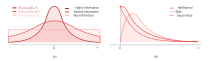
\includegraphics[width=1.0\textwidth]{images/ch3_informative_priors/informative_priors.png}
    \caption{Types of priors}
    \label{fig:priors}
\end{figure}

\subsection{Evidence} 

Also known as \textit{marginal likelihood}, it represents the probability of observing the data considering all possible parameter values. It is called marginal likelihood because it corresponds to the marginal probability calculated as the integral of the joint probability $P(data|\theta)$ across all $\theta$'s, as represented in \Cref{eq:marginal_likelihood}\citep{Lambert2018}. 

\begin{align}\label{eq:marginal_likelihood}
\begin{split}
    P(data)&=\int_{all \theta} P(data|\theta)\cdot P(\theta)d\theta  \\ 
    &=\int_{all \theta} P(data, \theta)d\theta
\end{split}
\end{align}

Although \Cref{eq:marginal_likelihood} is the formal definition, the marginal likelihood has an additional interpretation. Given that the likelihood function is not a probability distribution, it is expected that the multiplication of the likelihood by the prior is not either. Therefore, as the posterior needs to be a probability distribution, the marginal likelihood is the normalization factor that scales the numerator, so the area under the posterior distribution sums up to 1. Under this interpretation, the numerator in the Bayes theorem provides the shape of the posterior, while the Marginal Likelihood scales it out\footnote{This abstraction is key to introduce the sampling methods reviewed in \Cref{section:MCMC}}. 

The calculation of \Cref{eq:marginal_likelihood} can be trivial for simple models, but it becomes intractable for some real problems that include several parameters. This is one of the reasons why most of the Bayesian inference must be addressed using sampling methods instead of exact calculation. This will be reviewed in more detail in \Cref{section:MCMC}

\subsection{Posterior} 

Finally, applying the Bayes theorem to update the priors based on the evidence results in the posterior distribution. The posterior represents the updated probability distribution of our model's parameters and consolidates the knowledge of our system that was extracted from the data and the priors. 

While the Frequentist approach produces a point estimate for each parameter in the model, the Bayesian approach produces a probability distribution for each parameter, representing the uncertainty over the estimated model parameters. Then, point estimates such as mean, median, mode, and interval estimates can be calculated from this distribution. 

Although the point estimates produced by Frequentist and Bayesian approaches can be similar, there is a difference in the interval estimates produced by both approaches. In the Frequentist approach, the confidence interval (CI) is an interval of plausible values of a population parameter with a certain level of confidence constructed over many repeated experiments \citep{Devore2016}. For instance, a 95\% confidence level implies that if an experiment is repeated many times, 95\% of the samples will produce a CI that contains the true population parameter. Therefore, the confidence interval is a measure of the uncertainty over the interval, not over the parameter estimation \citep{Lambert2018}. 

In the Bayesian counterpart, the credible interval is a range that contains the true value of a population parameter with a particular probability. For instance, a 95\% credible interval means that the given range contains the true value with a probability of 95\%. Conversely to the Frequentist counterpart, the credible interval is a measure of the uncertainty over the estimation parameter. This interpretation of interval estimates seems more intuitive than the Frequentist confidence interval because it provides a probability over the parameters of interest. 

\section{Applying Bayes theorem: Markov Chain Monte Carlo sampling }\label{section:MCMC}

As discussed in the last section, the calculation of the denominator in the Bayes theorem complicates the application of Bayesian inference to real problems. The solution is to abandon the idea of exact calculation and use alternative methods to estimate the posterior distribution. One approach is to sample from the distribution to build an approximation; however, the posterior is still unknown until we can solve the denominator. 

Coming back to the idea that the numerator of the Bayes theorem provides the shape of our posterior and the denominator is a scaling factor, we can rewrite the Bayes theorem as: 


\begin{align}\label{eq:bayes_numerator}
\begin{split}
    P(\theta|data)&=\frac{P(data|\theta)\cdot P(\theta)}{P(data)}\\
    P(\theta|data) & \propto P(data|\theta)\cdot P(\theta)\\
\end{split}
\end{align}

In \Cref{eq:bayes_numerator}, the posterior is proportional to the multiplication of the likelihood function and the prior. Given that both terms in the numerator are known\footnote{Priors are defined by the modeller and likelihood is calculated based on the model choice and the observed data}, it is possible to sample from this function even if the denominator is unknown (it is not normalized), as shown in \Cref{fig:scalling_posterior}. 

\begin{figure}[H]
    \centering
    \includegraphics[width=1.0\textwidth]{images/ch3_scaling_posterior_space/scaling_posterior.png}
    \caption{Effect of scaling factor in the posterior space}
    \label{fig:scalling_posterior}
\end{figure}

This sampling process uses a method known as Markov Chain Monte Carlo (MCMC), which allows the approximation of a probability distribution by obtaining a sequence of random samples. The following section briefly introduces one algorithm within the MCMC family called Hamiltonian Monte Carlo (HMC), which is used in the development of this thesis. For further details of this algorithm, please review \citep{Lambert2018} and \citep{Neal2012}.

\subsection{Sampling from posterior: Hamiltonian Monte Carlo }

As the objective of the sampling process is to approximate the shape of the posterior distribution in \Cref{eq:bayes_numerator} (also known as \textit{posterior space}), different approaches such as rejection sampling, Gibbs sampling, or a simple Random Walk sampling can be used. However, these techniques are inefficient because they do not consider the shape of the distribution\footnote{An efficient sampler produces more samples from areas in which the posterior peaks (high probability density) and fewer samples from the rest of the distribution.}. 

The \textit{Hamiltonian Monte Carlo} method (HMC), a special case within the family of Markov Chain Monte Carlo (MCMC) algorithms, explores the posterior space more efficiently by using an analogy of a physical system in which a frictionless particle is moving around this space. In this physical system, two forces interact with the particle: gravity and the initial random momentum\footnote{This is the initial random impulse the particle receives that allows it to explore the posterior space.}. As the system is frictionless, the particle's position can be obtained at any time based on the previous position and the momentum applied to the particle \citep{Gelman2013,Lambert2018,McElreath2016,Neal2012}. 

To begin with, the posterior space is transformed into the negative log of the posterior $-log[(P(data|\theta))\cdot P(\theta)]$, also known as NLP space. This transformation converts all the peaks in the posterior space (zones with higher probability density) into valleys and the valleys in the posterior space (zones with lower probability density) into peaks. The idea behind this transformation is that the particle will visit more often the valleys of the NLP space because of the gravity effect. Therefore, more samples are taken from the zones with high probability density in the posterior space. \Cref{fig:nlp_space} shows a representation of the posterior and NLP space. It is important to highlight that the dimension of the NLP space is equal to the number of parameters in our model. So, the coordinates in this space are the model parameters. 

\begin{figure}[H]
    \centering
    \includegraphics[width=1.0\textwidth]{images/ch3_NLP_space/nlp_space.png}
    \caption{Sampling from the posterior distribution and the NLP space }
    \label{fig:nlp_space}
\end{figure}

After this transformation, the initial position of the particle ${\theta_{o}}$ is randomly initialized\footnote{${\theta_{o}}$ is a vector of coordinates in the posterior space} and the following iterative process starts:

\begin{itemize}
    \item First, an initial momentum is applied to the particle to start the process. This momentum is sampled from a multivariate normal distribution $m \sim \mathcal{N}(\mu, \scriptsize{\sum}\normalsize)$. Usually, this distribution is centred at zero with a diagonal covariance matrix.

    \item With this initial push, the particle will move through the sample space for a predefined amount of time $T$\footnote{This parameter is associated with the convergence of the algorithm. For instance, a smaller $T$ will better explore the NLP space but it will take longer to converge}. Then the new position ${\theta_{1}}$ and the momentum at that position $m_1$ are saved\footnote{In this part, the algorithm called \textit{leapfrog} solves the path of the particle moving over the NLP space using the Hamiltonian dynamics. For further explanation of this algorithm, please review \citep{Neal2012}}.

    \item With the initial and final position, the probability $r = \frac{P(X|\theta_{1})\cdot P(\theta_{1})}{P(X|\theta_{o})\cdot P(\theta_{o})}\footnotesize\times \normalsize\frac{q(m_1)}{q(m_o)}$ is calculated. In this expression:
    \begin{itemize}
        \item The first fraction is the ratio of the un-normalized posterior space at the initial and final position\footnote{The denominator in the Bayes theorem would have been cancelled in this expression because is the same for all places in the posterior space. Therefore, this is another explanation of why the denominator is not needed to sample from the posterior distribution.}.
        \item The second fraction is the ratio between the probability density function used to sample the momentum, evaluated at the initial and final position. This fraction allows the sampler to visit zones of lower probability (peaks in the NLP space) that otherwise would be rarely sampled because gravity biases our sampling to zones of higher probability.
    \end{itemize}
    \item A random number $u \sim Uniform(0,1)$ is generated. If $r>u$, position ${\theta_{1}}$ is accepted, and the particle will start the next iteration from that position; otherwise, the particle will return to ${\theta_{o}}$.
    \item Each accepted position ${\theta_{i}}$ is saved into a list. The sequence of ${\theta_{i}}$ samples is known as the sample chain. It is important to highlight that the accepted position ${\theta_{i}}$ corresponds to a set of samples of all model parameters because each coordinate in the posterior space corresponds to a parameter in the model. \Cref{fig:hmc} illustrates the sample-gathering process and details how the posterior distribution for each model parameter is built as the HMC algorithm explores the posterior space.    
\end{itemize}

\begin{figure}[H]
    \centering
    \includegraphics[width=1.0\textwidth]{images/ch3_hmc/hmc.png}
    \caption{Sampling process using the Hamiltonian Monte Carlo Algorithm}
    \label{fig:hmc}
\end{figure}

This iterative process is done in parallel for multiple chains to evaluate the sampling convergence and ensure that the posterior space is thoroughly sampled by starting in multiple random positions. The idea behind the multiple chains is that the posterior space will be better explored if each chain mixes well with other chains and does not get stuck in a single place, as shown in \Cref{fig:chains}. 

\begin{figure}[H]
    \centering
    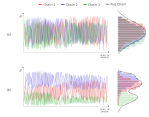
\includegraphics[width=1.0\textwidth]{images/ch3_chain_mix/chain_mix.png}
    \caption{Sampling using multiple chain exploration}
    \label{fig:chains}
\end{figure}

A common practice is to discard several iterations at the beginning of the process. These iterations are known as the warmup of the model and allow the chain to be stable before collecting the samples. Then, the sampling process is repeated multiple times until convergence is guaranteed. Convergence is measured by calculating the within- and between-chain variation, as proposed by \citet{Gelman1992},using the statistic $\hat{R}$ in \Cref{eq:r_hat}.

\begin{equation}\label{eq:r_hat}
    \hat{R} = \sqrt{\frac{W+{\frac{1}{n}}(B-W)}{W}}\\
\end{equation}

\begin{equation}
    W = \frac{1}{m}\sum_{j=1}^{m}s_{j}^{2}\ \ \ \ \ \ \ ; \text{with} \ \ s_{j}^{2}=\frac{1}{n-1}\sum_{i=1}^{n}(\theta_{ij}-\bar{\theta_{j}})^2
\end{equation}

\begin{equation}
    B=\frac{n}{m-1}\sum_{i=1}^{m}(\bar{\theta_{j}}-\bar{\theta})^2
\end{equation}

Where, $W$ is the within-chain variance, $s_j^2$ is the estimator for the sample variance for $j$-th chain, $n$ is the number of samples, $m$ is the number of chains, and $B$ is the between-chain variance. A common rule of convergence is that the statistic $\hat{R}$ should be below 1.01 for each model parameter.

For the analysis performed in this document, a variant of the Hamiltonian Monte Carlo algorithm is used to increase the sampling efficiency. This variant is known as the No U-Turn Sampler (NUTS) and follows the same principles as HMC but dynamically adapts $T$ to increase the sample's acceptance rate.

\subsection{Posterior predictive distribution }

The last section focuses on the use of MCMC methods (HMC in particular) to estimate the posterior distribution of model parameters, which can be used to draw conclusions or perform hypothesis testing. However, the real power of the model is when it is used to predict values in the light of new data. After HMC or any other MCMC algorithm is used to estimate the parameter posterior distributions, these posteriors can be used for prediction. 

The prediction in the Bayesian inference is performed using the following steps, also illustrated in \Cref{fig:posterior_pred}. Although this example corresponds to a univariate linear regression model with one intercept and one slope as model parameters, these steps can be applied in the same way to the multivariate case or any non-linear model: 

\begin{itemize}
    \item Samples from the posterior distribution of the intercept and the slope are collected. 

    \item Each set of parameter samples (intercept-slope) is used to calculate a regression line that produces a new target value. 
    
    \item These target values are known as the \textit{Posterior Predictive distribution}, which is the posterior distribution of the target variable\footnote{Posterior predictive refers to the distribution of the target variable whereas posterior refers to the parameter's distributions.}. 
\end{itemize}

\begin{figure}[H]
    \centering
    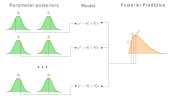
\includegraphics[width=1.0\textwidth]{images/ch3_posterior_pred/posterior_pred.png}
    \caption{Posterior predictive calculation process}
    \label{fig:posterior_pred}
\end{figure}

Once estimated, the posterior predictive distribution is helpful for several use cases: 

\begin{itemize}
    \item In hypothesis testing:
    \begin{itemize}
        \item Compare the posterior distribution within different groups to infer some characteristics from the population of interest. For instance, to measure the gender gap in salaries, the posterior predictive distribution of salaries between men and women can be compared to check the differences and magnitudes. 
    \end{itemize}
    \item For prediction: 
    \begin{itemize}
        \item Calculate point accuracy metrics for the target, such as Mean Squared Error (MSE), Root Mean Squared Error (RMSE), and Mean Absolute Percentage Error (MAPE). 

        \item Evaluate the model accuracy and performance in both in-sample and out-of-sample scenarios by comparing the posterior predictive distribution with the true distribution. 
        
        \item Calculate credible intervals for both the parameters and the target variable to estimate the uncertainty over the target variable through the predictive quantiles (\textit{k-th Percentile of prediction}) 
    \end{itemize}
    \item For simulation:
    \begin{itemize}
        \item Simulate new data that follows the sample distribution of the target variable (in-sample distribution) 

        \item Simulate hypothetical scenarios by changing the parameter's distributions and calculate their effect on the target variable, assuming that the same distribution governs the process. For instance, in the case of testing the impacts of a policy change on the gender gap, assessing the effects on salaries. 
    \end{itemize}
\end{itemize}

\section{Goodness-of-fit and predictive accuracy }\label{section:goodness_of_fit}

Once model parameters are inferred, it is necessary to measure how well the model represents the observed data (in-sample) and its predicting power on new data (out-of-sample). As reviewed in the posterior section, several point estimate metrics, such as MSE, RMSE, and MAE, can measure the model's predicting power. However, as Bayesian predictions are probability distributions, alternative methods that compare the true and the estimated distributions are preferred, as shown in the following subsections. 

\subsection{The ideal measure: Kullback-Leibler Divergence }

Using the theoretical foundations from information theory, the Kullback-Leibler divergence, also known as KL divergence, provides an ideal measure of the discrepancy between two distributions. It measures how much information is lost by using an alternative distribution instead of the true distribution \citep{Lambert2018}. This measure calculates the “distance” between the true distribution $p(x)$ and the alternative distribution $q(x)$, as shown in \Cref{eq:kl_divergence}. In this expression, if the distributions $p(x)$ and $q(x)$ are the same, the $KL$ will be 0. Then, the objective is to build a model that minimizes the $KL$ value.

\begin{align}\label{eq:kl_divergence}
    KL(p \rightarrow q) &= \int_{x \in X} p(x) \log\left(\frac{p(x)}{q(x)}\right) dx \\
    &= \underbrace{\int_{x \in X} p(x) \log(p(x)) dx}_{\text{true distribution}} - \underbrace{\int_{x \in X} p(x) \log(q(x)) dx}_{\text{estimated distribution}}\label{eq:kl_divergence_2} 
\end{align}

The KL divergence can be rewritten as in \Cref{eq:kl_divergence_2}, in which the first term is fixed because it is only related to the true distribution, while the second term is related to the model's choice. Given that the first part is fixed, the KL divergence will be minimized when the second term is maximized. 

In practice, the calculation of the complete KL divergence can be computationally expensive, given the integral calculations. Hence, the second term in the KL divergence can be used as a proxy to reduce the KL divergence using samples from the posterior predictive distribution. This term, also known as \textit{expected log-pointwise predictive density (elppd)}, is the base for comparing the performance between models and calculating some accuracy measures such as the WAIC and LOO-CV.

\subsection{Widely Applicable Information Criterion (WAIC) }

One estimate of the \textit{elppd} can be calculated by summing up the log of the average value of the likelihood across the posterior distribution for each data point $y_i$ used to estimate the model \citep{Gelman2013}, as shown in \Cref{eq:WAIC}. \citet{Gelman2013} recommends applying a \textit{bias} correction term that accounts for the uncertainty in the parameter estimation, and it serves as a regularization term that penalizes the model complexity.

\begin{equation}
    \widehat{elppd} = \sum_{i=1}^{n} \log \left[ E_{\text{posterior}}\left(p(y_i|\theta)\right) \right] - \underbrace{\sum_{i=1}^{n} \text{Var}_{\text{posterior}}\left(\log\left(p(y_i|\theta)\right)\right)}_{\text{bias correction}} \label{eq:WAIC}
\end{equation}

Then, the WAIC score is calculated as $WAIC= -2⋅ \widehat{elppd}$. The lower the WAIC, the better predictive performance of the model18. This score can also be used in model comparison to select the model with the best predictive power. As the WAIC score is calculated with the data points used in the model estimation, it is usually used to measure the model's in-sample predictive power. Nevertheless, if the dataset is split into training, validation, and testing, WAIC calculation using the test set can measure the model's out-of-sample predictive power.

\subsection{LOO-CV} 

Using the basic principle discussed in KL divergence, the method of Leave-one-out cross-validation allows the calculation of the model's out-of-sample predictive power by estimating the model with the $n-1$ data points and calculating the $\widehat{elppd}$ for the remaining datapoint to test the model's performance. The LOO-CV score will be the average of all $\widehat{elppd}$. This approach could be computationally expensive for large datasets, as the model will be re-estimated many times. 

\citet{Vehtari2015} propose an approximation to the LOO-CV score using samples from the posterior distribution estimated with the entire dataset. Therefore, the model will be estimated just once. This method is known as \textit{Pareto Smoothed Importance Sampling (PSIS)}. 

\section{Probabilistic programming: A framework to perform MCMC }

In practice, Bayesian inference is performed using a programming paradigm called Probabilistic programming. This approach combines traditional programming languages with probability theory to handle uncertainty in the modelling process. The general idea in probabilistic programming is that a model corresponds to a series of interconnected random variables, and all calculations are performed using a graph structure. 

There is an ample supply of packages that ease the application of the Bayesian inference framework. Given the author's familiarity with the programming language Python, this thesis uses Numpyro \citep{Phan2019} as the inference library. One interesting characteristic of Numpyro is that it uses JAX for the sampling process. JAX is a powerful library for efficiently performing numerical computation and tensor operations in CPUs, GPUs, TPUs and other multi-device environments. This characteristic is critical given the computational cost of performing Bayesian inference. 